\documentclass[tikz,border=15pt]{standalone}
\usepackage{circuitikz}
\begin{document}
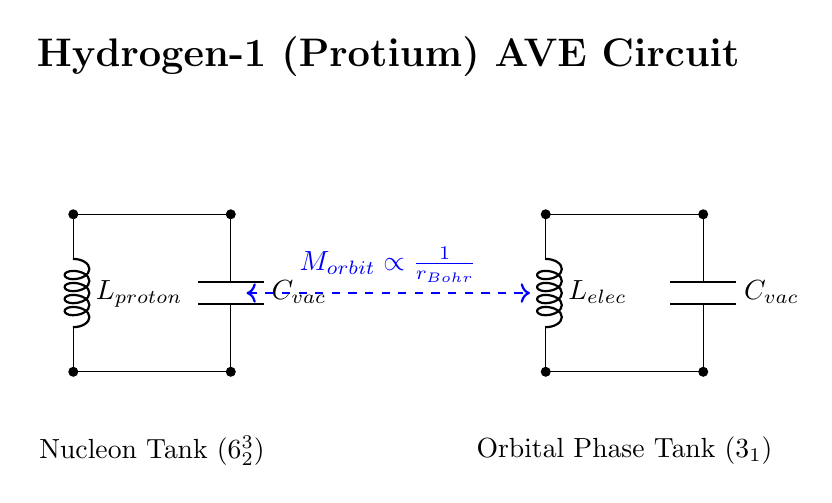
\begin{tikzpicture}
    \begin{scope}[shift={(0,0)}]
        \draw (0,0.5) to[L=$L_{proton}$, *-*] (0,-1.5);
        \draw (2,0.5) to[C=$C_{vac}$, *-*] (2,-1.5);
        \draw (0,0.5) -- (2,0.5);
        \draw (0,-1.5) -- (2,-1.5);
        \node at (1, -2.5) {Nucleon Tank ($6^3_2$)};
    \end{scope}

    \begin{scope}[shift={(6,0)}]
        \draw (0,0.5) to[L=$L_{elec}$, *-*] (0,-1.5);
        \draw (2,0.5) to[C=$C_{vac}$, *-*] (2,-1.5);
        \draw (0,0.5) -- (2,0.5);
        \draw (0,-1.5) -- (2,-1.5);
        \node at (1, -2.5) {Orbital Phase Tank ($3_1$)};
    \end{scope}

    \draw[<->, dashed, blue, thick] (2.2,-0.5) -- (5.8,-0.5) node[midway, above] {$M_{orbit} \propto \frac{1}{r_{Bohr}}$};

    \node at (4, 2.5) {\Large \textbf{Hydrogen-1 (Protium) AVE Circuit}};
\end{tikzpicture}
\end{document}
